\documentclass[12pt]{report}
\usepackage[margin=1.2in]{geometry}
\usepackage{fancyhdr}
\usepackage{framed, color}
\usepackage{graphicx}
\usepackage{url}
\usepackage{mathtools}  
\usepackage{amsmath}
\usepackage{amssymb}
\usepackage{tabulary}
\usepackage{booktabs}

\title{\textbf{Video Classification using Consensus Learning and CrowdSourcing}}
\author{
		\bf{B.Tech. Project Phase I Report}\\
        \\
        \emph{Submitted in partial fulfillment of requirements for the degree of}\\
        \bf{Bachelor of Technology}\\
        \\
        \emph{by}\\
		\bf{Aditya Kumar Akash}\\
        \bf{Roll No : 120050046}\\
        \\
        \emph{under the guidance of}\\
		\bf{Prof. Ganesh Ramakrishnan}\\
        \\\\
        
\includegraphics[height=3.5cm]{./iitb_logo.jpg}\\
        \\
		\bf{Department of Computer Science and Engineering}\\
        \bf{Indian Institute of Technology Bombay}\\
        \bf{Mumbai 400076, India}\\
}
\date{November, 2015}

\bibliographystyle{plain}

\begin{document}
\maketitle
\pagebreak
\tableofcontents
\pagebreak

\begin{abstract}
A video conveys a lot of information about any subject than a mere picture. We currently have a huge collection of videos. So classification of the videos would help in easy and fast location of video of interest, saving time and also serving as a learning tool. In this work we work towards assigning tags to videos using crowd sourcing.

Crowd sourcing using games are one of the methods currently used to gather data in a fast and cheap way. The game interface asks player to tag the videos, for which he would be awarded points based on a scoring mechanism. We improve the existing scoring and try to build a metalearner which would be learning about tags and videos and serve as video classifier.
 
Meta learners based on ensemble models are popular choice for multi label multi class classifiers. Amongst different meta learners  consensus learning best suits our framework. We use MLCM, a simple consensus learning model to achieve the task at hand.
\end{abstract}
\pagebreak

\renewcommand{\abstractname}{Acknowledgements}
\begin{abstract}
My sincere thanks to Prof. Ganesh Ramakrishnan for providing valuable feedback time and again which served to influence and improve this work.

I would also like to thank the entire team: Dr. Simoni S.Shah, Post-Doctoral Fellow IIT Bombay,and my fellow team mates Depen Morwani, Saketh Vadlamudi, Shraddha Bhattad, Deepak Dilipkumar for their extended discussions and brainstorming on various issues.

Special thanks to Ashish Kulkarni, Research Scholar at IIT Bombay and Mitesh Khapra, Researcher India Research Laboratory, Bangalore, India for providing us valuable insights.

I would also like to thank Ankit Vani \& Pooja Ahuja, Interns at IIT Bombay for designing the initial game framework.
\end{abstract}
\pagebreak

\chapter{Introduction}
\section{Motivation}
Video is a powerful tool to convey any information precisely. Looking at an action frame by frame with audio providing supporting explanation is highly informative and easier to grasp. This makes video a popular choice for learning new concepts. 

Video is both appealing and intelligible to masses and that makes it an medium for instruction. Using videos farmers can stay in touch with the latest technology, success stories of other farmers around the world. A video library can easily be accessed and utilized by farmer groups using specialized mobile applications, as smart-phones have now become common. A farmer can learn from a relevant video and solve his problem without an actual expert present to guide him. The aim of this project is to facilitate such a video library where suggestions of relevant videos be made to farmers to help them solve their problem. 

Present video repositories like \emph{YouTube} have collection of videos which serve general purpose video classification. We need a classification which more suits an agriculture domain and hence it forms a closed domain. Moreover manual video collection and tagging is a tedious task. Thus we seek to use crowd sourcing as an option for video collection as well obtaining tags. 

In order to attract people to participate in such a crowd sourced activity voluntarily they must be given some incentive as such a fun element. So we introduce \emph{Video Tagging} game where users can watch the videos and provide tags for which they are given points. In this way they both enjoy the game as well as learn from it. As a result of users interacting with the game we obtain rich collection of tags which we use to predict the relevant tags of the videos. This brings in meta learner models which learn association of tags to videos which would also help in recommendation of videos and easy navigation.

\section{Related Work}
Researchers have attempted to achieve video classification. However either they only utilize the meta data of video, audio and text or require computationally expensive models to solve the problem. Some of the algorithms consider entire video as a single feature vector and approach
this problem from the aspect of co-training multiple complementary views.

\emph{VideoKheti}\cite{videoKheti} attempts to present agricultural videos to farmers. However in this the main aim was not to categorize videos, but to acquire data on the user experience and the usability of multi-modal interaction system for searching and viewing of agricultural videos.

Active learning has been used to evolve personalized category catalogue for agricultural videos in \cite{AMN}. However they use associative Markov networks which are computationally expensive and so inappropriate from game point of view. 

\emph{VideoMule}\cite{videoMule} combines individual classification and clustering algorithms trained on textual meta-data, audio and video through a heuristic consensus based learning. However, they have no crowd sourcing element hence they would not have evolving tag set for a given video. This is because interpretation of information present in video changes over time.

\emph{BGCM}\cite{BGCM} deals with single label multiclass classification, such that prediction combination happens within the individual labels. We could apply this method to multi label multiclass classification by combining predictions of base models for each label, resulting in consolidated predictions for each label. Then the consolidated predictions are collected to get the final prediction. But these could not capture label correlations.
 
In this work, we try to achieve video classification for agricultural domain we use a crowd sourcing based approach of tag collection. We first look at how to rank the tags based on simple tf-idf scoring. We then combine them using a consensus based model. We adapt the consensus method presented in \cite{MLCM} to generate multiple semantic labels to the videos. This approach has less computational cost and also is based on crowd sourced data, and hence the assigned tags evolve with time. 
 
\chapter{TagVideo Game}
\section{Working of the Game}
The \emph{tagVideo} game allows user to play videos and while the video plays they can start typing a tag and get a list of suggestions. The user selects from these selections and gets scored for it. The user can end the game and submit the score at any time. In the figure below we can see scores for different tags user has entered.

\begin{figure}[h!]
\centering
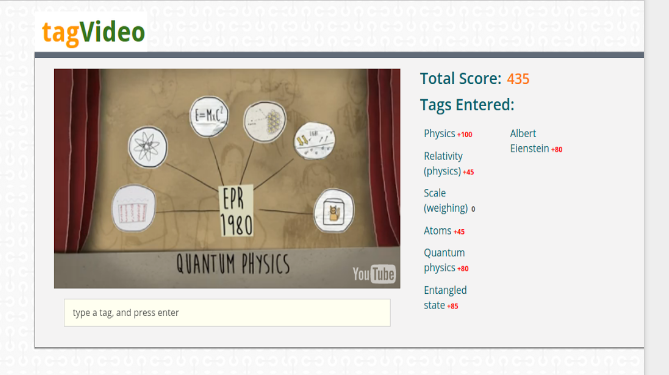
\includegraphics[width=1.0\textwidth]{tagVideoGame.png}
\caption{TagVideo Game in action}
\end{figure}

Based on the scores cumulative across all the videos the user is ranked against other users. This introduces competitiveness to give better tags for the videos and keeps the user attentive.

\begin{figure}[h!]
\centering
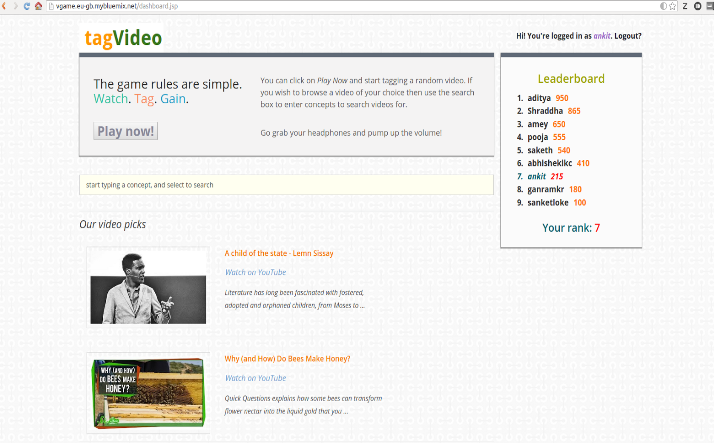
\includegraphics[width=1.0\textwidth]{tagVideoDashboard.png}
\caption{TagVideo game Dashboard}
\end{figure}

The above image shows dashboard for a given player and the global rank list on the right. User can also search for videos of his interest or click on \emph{PlayNow} to watch a random video from the library.

This initial game framework was developed by Ankit and Puja. We next investigate the function they have used for generating the scores of the tags entered.

\pagebreak

\section{Existing Scoring Function}
Providing scores to the tags is at the heart of this game. It keeps the player motivated to play the game as well as provide better and relevant tags in order to get better scores. The scoring function can be also viewed as an outcome of a hidden model which associates the tags to videos and generates a relevance score. Thus a good scoring function suggests a good model, and hence a good classification of videos.

All the videos are initially fed into \emph{IBM Watson Concept Insight Corpus}. When the player starts typing a tag, we use IBM Watson Concept Insights to auto-complete and suggest possible tags. When the user selects a tag, we score based on the \emph{IBM Watson Concept Insights relevance score} of the tag with the video. Scoring is based on how relevant a given tag is to a video.

Initially, this score is purely based on the relevance score returned by IBM Watson Concept Insights
As more and more users tag a video, a \emph{TF-IDF component} of the scoring function starts gaining more weight.We assume that tags that more people agree on are correct. Thus, if for a given video, a large number of people have given a tag, it gets a higher score. Inversely, if that tag is common in many other videos, its score for this video diminishes. This principle encourages more specific tags, inducing greater focus on the video.

Lets see the scoring function in detail.

\begin{table}[htbp]\caption{Notation of Tf-Idf Scoring}
\begin{center}% used the environment to augment the vertical space
% between the caption and the table
\begin{tabular}{r | p{10cm} }
\toprule
Symbol & Meaning\\
\hline
$t$ & Tag\\
$v$ & Video\\
$f^t_v$ & Frequency of tag $t$ in video $v$\\
$tf$ & Term Frequency\\
$c_v$ & Count of distinct tags given for video $v$\\
$N$ & Total Number of videos in library\\
$N_t$ & Number of videos in which tag $t$ appears\\
$idf$ & Inverse Document Frequency\\
$s_{watson}$ & Score for a tag by IBM Watson\\
$w_{watson}$ & Weight for Watson score\\
$N_v$ & Count of number of users who tagged video $v$\\
$tf\_idf$ & Tf-Idf score for a tag video pair\\
\bottomrule
\end{tabular}
\end{center}
\label{tab:TfIdfNotation}
\end{table}

Now we have, the term frequency which denotes in comparison to other tags how relevant is this tag for the given video,
\begin{equation}
tf = \frac{f^t_v}{c_v}
\end{equation}
Then Inverse document frequency which denotes how specific the tag is for the video. It is inversely related to how spread the tag is across video library.
\begin{equation}
idf = 1 + \log\frac{N}{N_t}
\end{equation}
The TF-IDF component of score,
\begin{equation}
tf\_Idf = tf * idf
\end{equation}
The weight given to watson score is decreased with increase in number of taggers for a given video. This is done to shift on consensus of people to decide the relevant tag,
\begin{equation}
w_{watson}=\frac{1}{e^{c_0*(N_v - 1)}}
\end{equation}
The final score awarded to a tag for a video is given by -
\begin{equation}
score = s_{watson}*w_{watson}*idf*c_1 + (1-w_{watson}) * \frac{tf\_Idf}{max_t^v(tf\_Idf)} * c_2 + c_3
\end{equation}
where $max_t^v $ takes maximum value over tags for video $v$, and $c_0, c_1, c_2, c_3$ are constants which help to bring the score in range 1 to 100.
\pagebreak

\section{Analysis of Scoring Function}
The scoring function shifts the score from IBM Watson score towards some kind of consensus among users with more weights to video specific tags. This is a desired property since we want that the relevance of a tag be determined by the players of the game.

Some other properties which we expect a good scoring function to follow are -
\begin{enumerate}
\item It should not be possible for users to co-ordinate and game the system. This means that users should not communicate and provide same tags to get high scores by virtue of term frequency.
\item Global strategy amongst users to provide junk tags eg. abc, xyz should not work. There could be a website or public forum where users decide upon a global strategy to provide some given tags irrespective of the video they are watching. The scoring function should nullify such cases.
\end{enumerate}
We only allow those tags to be specified which are present as a concept in \emph{Wikipedia}. This ensures that junk would not be a part of tag set for any video. The factor of $\frac{tf\_idf}{max_t^v(tf\_idf)}$ because of division by maximum $tf\_idf$ ensures that after sufficient number of good tags have been collected for a given video the effect of junk tags and gaming the system is negligible.
\vspace{1em}\\
But \emph{this scoring function has certain inherent problems}. These are - 
\begin{enumerate}
\item In calculating term frequency, $tf=\frac{f_v^t}{c_v}$, division by count of distinct tags is not necessary since this gets canceled out in the final score calculation
\item Presence of $\frac{tfIdf}{max_v(tfIdf)}$ factor is just to get score in range (0, 1). This demands extra information to be stored
\item In factor $\frac{tfIdf}{max_v(tfIdf)}$ = $\frac{tf_1*idf_1}{tf_2*idf_2}$, let subscript 2 corresponds to max value $tf\_idf$. Let tag $2$ denote a relevant tag and tag $1$ a unrelated tag. Now $idf_2$ can be reduced by tagging other videos with tag $2$, thus increasing $N_t$, which would cause increase in score for some unrelated tag $1$, which is not used for other videos, thus having higher $idf_2$. This is not desirable.
\end{enumerate}
\vspace{2em}

We try to improve upon the scoring function while preserving the desired properties.
\pagebreak

\section{Improvement of Scoring Function}
We improve upon some of the components of the scoring function -
\begin{enumerate}
\item Term frequency is changed as $tf=\frac{f_v^t}{f_v}$. Division by maximum frequent tag ensures that $tf$ of an unrelated tag would decrease as we have sufficient number of related tags.
\item Instead of normalization by division using $max_t^v(tf\_idf)$, we use division by $1 + log{N}$
\item Above $tf$ and normalization ensure TF-IDF scores between 0 and 1 along with property that unrelated tag scores decreases with increase in sufficient number of related tags.
\end{enumerate}
\vspace{1em}

The new term frequency would be -
\begin{equation}
tf = \frac{f^t_v}{max_v(f_v^t)}
\end{equation}
where $max_v$ takes maximum value of frequency for the video $v$.\\
The new normalization term would be -
\begin{equation}
idf_{max} = 1 + \log N
\end{equation}
Other values being same from the old scoring, the new scoring function becomes -
\begin{equation}
score = s_{watson}*w_{watson}*\frac{idf}{idf_{max}}*c_1 + (1-w_{watson}) * \frac{tf\_Idf}{idf_{max}} * c_2 + c_3
\end{equation}

This new scoring function overcomes the problems we specified in the previous section 2.3. 
\begin{enumerate}
\item There is no term which is cancelled out in this function and hence no unnecessary computation.
\item The normalization factor is a constant and cannot be influenced.
\item The new scoring function has desired properties from the previous scoring function and hence is good.
\end{enumerate}
\vspace{1em}
We next demonstrate the effect of both the functions over small data-set.

\pagebreak

\section{Experiments and Results}
In the experimental setup we have users $S1$ to $S9$. Users go on to tag two videos with two tags - one relevant and other irrelevant. In one case the score is given by old scoring and in other case using the new scoring.\\
\vspace{1em}\\
\textbf{Old Scoring} : 
After user \textbf{S4} completes tagging 9 different videos where tagged \emph{Iron Man}, then user \textbf{S5} onward proceeded to re-tag this video.

\begin{table}[!h]
\begin{center}

  \begin{tabular}{l l l l l l l l l l}
  \toprule
  \textbf{Tag} & \textbf{S1} & \textbf{S2} & \textbf{S3} & \textbf{S4} & \textbf{S5} & \textbf{S6}& \textbf{S7} & \textbf{S8} & \textbf{S9}\\
  \midrule
  Iron Man & 80 & 100 & 100 & 100 & -  & -  & 100 & 100 & -  \\
  Metal    & 0  & 10  & -   & -   & 40 & 90 & -   & -   & 100\\
  \bottomrule
  \end{tabular}
	\caption{Variation of Tag Score for Video - Will you be iron man?}

\end{center}
\end{table}

\vspace{2em}
\textbf{New Scoring} :
After user \textbf{S4}, 9 different videos where tagged \emph{Food}, then users \textbf{S5} onward proceeded to re-tag this video.

\begin{table}[!h]
\begin{center}

  \begin{tabular}{l l l l l l l l l l}
  \toprule
  \textbf{Tag} & \textbf{S1} & \textbf{S2} & \textbf{S3} & \textbf{S4} & \textbf{S5} & \textbf{S6}& \textbf{S7} & \textbf{S8} & \textbf{S9}\\
  \midrule
  Food & 70 & 75 & 90 & 100 & -  & -  & 95 & 95 & - \\
  Shoe & 0  & 0  & -  & -   & 20 & 60 & -  & -  & 75\\
  \bottomrule
  \end{tabular}
	\caption{Tag Score for Video - Science of sweetness}

\end{center}
\end{table}
'-' denotes this tag was not given

\emph{\textbf{Observations} which reflect the improvements of new scoring function} - 
\begin{enumerate}
  \item The old scoring does not reflect clearly idf factor affecting the score. Even when 9 more videos where tagged with \emph{Iron Man} there is no change in its score in user \textbf{S7} in Table 2.2 . But we can see in Table 2.3 there is dip in score of tag \emph{Food}. Thus the new scoring function showing better sensitivity.
  \item Old scoring allows unrelated tags have spiked increase in score which can be observed in the higher rate of increase in score for tag \emph{Metal} with the number of tagging. The new scoring allows a gradual controlled increase and thus discourages users to given unrelated tags just to obtain higher scores.
\end{enumerate}
All these establish that the new scoring function has the desirable properties which we stated in section 2.3. \emph{The scoring function induces a ranking on the tags for a video}. Picking the tags after putting some threshold score would achieve video classification.
 
\chapter{MetaLearner}
\section{MetaLearners}
We have seen in the previous chapter how TF-IDF scoring is used to combine the tags users give in order to achieve the video classification. But it has certain shortcomings. 
\begin{enumerate}
\item There is no learning element involved. We just take the majority voting and account of specificity of the tags in order to rank the tags.
\item The TF-IDF model would only be able to suggest tags from the set of tags which people have suggested for a given video. 
\item No correlation between tags or domain knowledge is utilized in scoring the tags.
\end{enumerate}

We would like to now introduce some learning elements. We look for meta learning in this case because we do not have knowledge about the features the users looked into in order to give a particular tag set. We only have access to tag sets. Thus meta learners are perfect models for our problem.
\vspace{1em}\\

We remodel our problem, in order to be able to use meta learning algorithms. So we assume following -
\begin{enumerate}
\item Each user is a base learner. A user has undergone real life training in inferring relevance of tags and items, here videos. Based on his experience he gives tag set for a given video. We treat it as output of his base learner.
\item User gives tags from a fixed set of global tags. This keeps the tag set free of concepts which are not known.
\item Classifiers based on images and metadata from videos are another base learner along with users.
\end{enumerate}

Keeping these assumptions in mind we explore most popular metalearners and select the one which best suit to our problem.

\section{Ensemble based Learners}
As we see our problem is closely related to multi label multi class classification, Boosting which is an ensemble based learner is a popular choice because of its theoretical performance guarantees and strong experimental results. Ensemble learners are based on utilizing multiple learning algorithms to consolidate their results. Our problem fits into this as we assumed users to be base learners.

Most of the boosting algorithms are adaptations of \emph{AdaBoost}\cite{AdaBoost} algorithm. So we analyze adaBoost to see possibility of using it in our setting.
\vspace{1em}\\
AdaBoost\cite{OnlineAdaBoost} generates a sequence of base models $h_1, h_2,...,h_M$ using weighted training sets (weighted by $D_1, D_2...,D_M$) such that the training examples misclassified by model $h_{m-1}$ are given half the total weight when generating model $h_m$ and correctly classified examples are given the remaining half of the weight. One of the major steps in this algorithm is calculation of weighted error for a base classifier, $h_m$, as - 
\begin{equation}
\epsilon_m = \sum_{i:h_m(x_i) \neq y_i}D_m(i)
\end{equation}
As we can see we need supervised data for training in this algorithm. Generating supervised data to train the model would require manual effort, since in our case we have crowd sourced data of video with tagset. Hence we abandon this idea of using adaboost based metalearners. 

We would ideally want learners which focus of combination of model outcomes with maximum agreement amongst the learners. This brings us to consensus based learners which we explore in our next section.
\pagebreak

\section{Consensus based Learning}
Combination of multiple models helps to overcome effects of poor data quality and also makes the final combined model more robust. In certain situation we may only have access to the predictions from the raw data and not the raw data itself. Consensus based prediction combination algorithms are effective for these situations. 

We adapt the MultiLabel Consensus Maximization for ranking MLCM-r from \cite{MLCM} to achieve consensus amongst different users for the tags of a given video. We shall call it MLCM. As per authors of \cite{MLCM} "MLCM-r consolidates the predictions of base models via maximizing model consensus and exploits correlations using random walk in the label space." Let us see MLCM-r :

\begin{table}[htbp]\caption{Notations for MLCM-r}
\begin{center}% used the environment to augment the vertical space
% between the caption and the table
\begin{tabular}{r | p{10cm} }
\toprule
Symbol & Meaning\\
\hline
$m$ & Number of multilabel classifiers\\
$n$ & Number of Instances\\
$l$ & Number of labels\\
$\boldsymbol{x}$ & An instance\\
$\|.\|$ & Frobenius Norm\\
$A$ & $a_{i,j}$ is the prediction of label $(j$ mod $l)$ on $\boldsymbol{x}_i$ by $\lfloor j/l \rfloor$\\
$B$ & Label node class distribution\\
$U$ & $u_{i,l}$ is the probability that label $l$ is relevant to $\boldsymbol{x}_i$\\
$Q$ & $q_{i,l}$ is the probability of seeing label $l$ given label $j$\\
\bottomrule
\end{tabular}
\end{center}
\label{tab:TableforMLCM}
\end{table}

We have predictions of $m$ classifiers for $n$ instances, with each prediction being a $l$ length tuple consisting of $0$'s and $1$'s, with $1$ at position $i$ meaning that the $i$th label is relevant to this instance. This information of prediction is encoded in matrix $A$, which is $n$ by $v$  $(v=m\times l)$, where $(i, (k - 1) \times l + j)$-th entry is $1$ if the $k$-th model predicts that the $j$-th label is relevant to the $i$-th instance, otherwise that entry is set to $0$. 

We construct a bipartite graph with $A$ as the connection matrix. The graph has $n$ instance nodes and $v = m \times l$ group nodes. A group node represents a label. The group nodes are annotated by letter $g$ and the instance nodes by letter $x$. An instance node can be connected to more than one group nodes from a single classifier, representing the multilabel predictions of that classifier. A dashed rectangle surrounds group nodes which belong to the same classifier. There is another layer of nodes called label nodes which help represent the label the group node stands for. An example graph has been shown in Figure 3.1 for 2 instances, 3 labels and 2 classifiers. 
\pagebreak

\begin{figure}[h!]
\centering
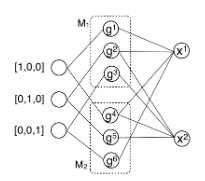
\includegraphics[width=0.3\textwidth]{MLCMgraph.png}
\caption{Bipartite Graph for MLCM-r\cite{MLCM}}
\end{figure}

Each node has a probability distribution associated with it. 
\begin{enumerate}
\item Each instance node $i$ is associated with probability distribution $\boldsymbol{u}_i$, where $u_{i, l}$ stands for probability of relevance of $l$-th label on $i$-th instance. Matrix $U=[u_1^{'},...,u_n^{'}]$ represents this information. 
\item Each group node $j$ is associated with probability distribution $\boldsymbol{q}_j$, where $q_{j, l}$ stands for probability of seeing label $l$ given $j$-th label. This relates to how related two labels are in opinion the the classifier to which the group node $j$ belongs. Matrix $Q = [q_1^{'},...,q_2^{'}]$ encodes this information.
\item Each group node $j$ representing label $l$ is also connected to label node which has probability distribution $\boldsymbol{b}_j$, where $l$-th entry is $1$ and others 0. Matrix $B = [b_1^{'},...,b_v^{'}]$ encodes this information.
\end{enumerate}

MLCM-r maximizes model consensus by solving the following optimization problem :
\begin{equation}
\min_{U, Q} \sum_{i=1}^n\sum_{j=1}^v a_{ij}\|\boldsymbol{u}_i - \boldsymbol{q}_j\|^2 + \alpha\sum_{j=1}^v\|\boldsymbol{q}_j-\boldsymbol{b}_j\|^2
\end{equation}
s.t.
\begin{equation}
u_{ik}\geq 0, \sum_{k=1}^l u_{ik} = 1, i = 1,...,n
\end{equation}
\begin{equation}
q_{jk}\geq 0, \sum_{k=1}^l q_{jk} = 1, j = 1,...,v
\end{equation}
In this the first term ensures that if an object $\boldsymbol{x}_i$ is linked to group $\boldsymbol{g}_j$, then their probability distribution should be similar since both of them in some sense represent probability of seeing label while being at that node. The second term ensures that the probability distribution of the groups does not deviate much from its initial distribution. $\alpha$ is the factor of how much we would like to penalize such a constraint violation.

The solution\cite{BGCM} is obtained by block co-ordinate descent :
\begin{equation}
\boldsymbol{q}_j^t = \frac{\sum_{i=1}^n a_{ij}\boldsymbol{u}_i^{t-1} + \alpha \boldsymbol{b}_j}{\sum_{i=1}^n a_{ij} + \alpha}
\end{equation}
\begin{equation}
\boldsymbol{q}_j^t=\frac{\sum_{j=1}^va_{ij}\boldsymbol{q}_j^t}{\sum_{j=1}^va_{ij}}
\end{equation}
Upon convergence, the final probability distributions are given in the rows of $U$. Most likely label can be decided from this.
\vspace{1em}\\
We adapt this setting for our problem of classifying video. Our analogy consists of
\begin{enumerate}
\item A video is considered an instance $\boldsymbol{x}$
\item Each user is considered as multilabel classifier, since the users watch the videos and give the tags
\item Tags are correspondence of labels. We had earlier limited the tags from a fixed set of $Wikipedia$ concepts which helps here.
\end{enumerate}
For cases when a person does not tag a video, we assume that he does not associate it with any of the labels, and fill the connection matrix with entry of $0$. After obtaining matrix $U$, we keep a threshold to obtain set of labels (tags) which are relevant to the given video.

Next we experiment with this algorithm on the data collected using the \emph{tagVideo} game and analyze the results.

\pagebreak
\section{Experiments and Results}
The experimental setting consists of $tagVideo$ game where users provide tag set for videos. We use the same analogy as described in previous section 3.3. We also use \emph{Kendall rank correlation coefficient} $\tau$ to measure the correlation between the rankings generated using TF-IDF scoring and MLCM-r scoring. The kendall's tau measures rank correlation: the similarity of the orderings of the data when ranked by each of the above method. This allows us to have a sense of how different MLCM-r becomes while it maximizes consensus.  

We present the results in two parts each bringing out certain facet of MLCM-r.\vspace{0.5em}
\textbf{CASE 1}\\
\begin{table}[htbp]\caption{Result Table 1}
\begin{center}% used the environment to augment the vertical space
% between the caption and the table
\begin{tabular}{p{3cm} | p{5cm} | p{5cm} | p{3cm}}
\toprule
Video Id & Tag-Score by TF-IDF & Tag-Score by MLCM-r & Correlation $\tau$\\
\hline
guh7i7tHeZk & 
\begin{itemize}
\item ScienCe,1
\end{itemize} & 
\begin{itemize}
\item ScienCe,0.49
\item Technology,0.26
\item Play \& Win,0.26
\end{itemize} & 0.67\\
\hline
mtg9p6A6xnY & 
\begin{itemize}
\item Element 13,0.54
\item Periodic Table,0.46
\end{itemize} & 
\begin{itemize}
\item Element 13,0.41
\item Periodic Table,0.36
\item Chemistry,0.23
\end{itemize} & 1.0\\
\hline
w2Qk-jz\_tWc &
\begin{itemize}
\item Animals,1
\end{itemize} &
\begin{itemize}
\item Animals,0.38 
\item Irrigation,0.15 
\item Crops,0.15 
\item Food,0.15 
\item Farming,0.15
\end{itemize} &
0.4\\
\bottomrule
\end{tabular}
\end{center}
\label{tab:ResultTable1}
\end{table}
\vspace{1em}\\
We obtain following observation from Table 3.2 :
\begin{enumerate}
\item TF-IDF is only capable of ordering tags which where actually assigned to the video by the users.
\item MLCM-r also provides new tags which are related to original tags. Thus MLCM-r shows its capacity to capture label correlations. Correlations lead to appearance of tags like \emph{Chemistry} with \emph{Periodic Table}, even when no user had specified \emph{Chemistry} as a tag.
\end{enumerate}

\textbf{CASE 2}\\
\begin{table}[htbp]\caption{Result Table 2}
\begin{center}% used the environment to augment the vertical space
% between the caption and the table
\begin{tabular}{p{3cm} | p{5cm} | p{5.2cm} | p{3cm}}
\toprule
Video Id & Tag-Score by TF-IDF & Tag-Score by MLCM-r & Correlation $\tau$\\
\hline
649iUqrOKuE & 
\begin{itemize}
\item Big data,1
\end{itemize} & 
\begin{itemize}
\item Big data,0.28 
\item CERN,0.21
\item Data storage,0.15
\item Cloud Computing,0.15
\item \emph{Tag (graffiti)},0.14
\item \emph{Tag (HTML)},0.07 
\end{itemize} & 0.33\\
\bottomrule
\end{tabular}
\end{center}
\label{tab:ResultTable1}
\end{table}
\vspace{1em}\\
Table 3.3 gives us following insight :
\begin{enumerate}
\item MLCM-r not only brings in additional related tags, but it also brings in unrelated tags (\emph{italicized in table 3.3}) which are profusely given with these related tags in some other videos.
\item The above limitation causes MLCM-r to provide a lot more tags than the optimal amount
\end{enumerate}
We obtain average correlation of $\tau=0.26$, which tells that it positively agrees with TF-IDF rank list.These results demonstrates capability of MLCM-r in capturing the label correlations, which help to bring in new relevant tags for the videos, while still maintaining good agreement with majority voting rank list.
\chapter{Conclusion and Summary}
\section{Summary}
In this work, we have looked into how to utilize crowd sourcing in order to achieve video classification, with main objective of helping the farming community. We saw \emph{TagVideo} game as an interface to collect data, and serving as a fun and learning element to players. We looked at the scoring mechanism and its improvements, so as to not allow users game the system.

We then introduced learning element into the game in form of metalearners. We analyzed popular metalearners and picked consensus learning for our problem. We then looked into working of MLCM-r and its improved tag prediction over TF-IDF. One application of MLCM-r apart from this problem could be in recommendation section, such as movie recommendation, where we need correlation between movies that users have watched.

It was a great learning experience to work on a problem with practical applicability. I learned a lot about metalearners, and had good experience of working in a group. 
\pagebreak


\section{Future Work}
In our work, we were able to use consensus learning algorithm, MLCM-r, to do video classification for crowd sourced data. But the method has limitations on which we would like to improve upon in our future work. The limitations with desirable improvements would be :
\begin{enumerate}
\item MLCM-r does allow for online updates, i.e. we need to compute the prediction from scratch in case some new edges are added. We would like to make the adapt the algorithm for online case to manage following :
	\begin{itemize}
		\item Handle the adding of new edges due to users tagging videos which they had not tagged previously	
		\item New users being added into the system
		\item Increase in number of tags. We would like our tag set to grow with time, so that we do not miss on new terms
		\item New videos being added to the system
	\end{itemize}
\item We have not utilized any domain knowledge. A prior knowledge graph containing the relations between tags is being currently built by fellow teammates, Depen and Shraddha. We would like to re-frame the optimization problem to be able to utilize the information. 
\item We also would like to separate tags from concepts. This would give freedom to users to express tags in more specific free forms. Deepak in looking into working of mapping tags to concepts. We would like to change our model to utilize this transformation.
\item We would also like to improve the complexity of the algorithm, to handle situations when our video library grows big, and the system has lots of users.
\item We would also like to model the trust factor of users to attach weights to the tags he would be giving.
\end{enumerate}


\textbf{Consensus Learning for entire platform :} \\
We would like to use consensus in all the platforms - Consensus amongst users to decide tags, consensus of tags predicted with the knowledge graph and consensus between user predicted tags and tags from algorithms based on textual and video, audio metadata.\\


These points summarize the future potential of the project.


\begin{thebibliography}{1}
%Dolor
\bibitem{MLCM} 
Sihong Xie, Xiangnan Kong, Jing Gao, Wei Fan, and Philip S. Yu. Multilabel consensus classification. In ICDM,2013.

\bibitem{BGCM}
Jing  Gao,  Feng  Liang,  Wei Fan,  Yizhou  Sun,  and  Jiawei  Han. Graph-based consensus maximization among multiple supervised and unsupervised models.  In NIPS, 2009

\bibitem{videoKheti} 
 S. Cuendet, I. Medhi, K. Bali, and E. Cutrell.
Videokheti:  Making video content accessible to
low-literate and novice users. ACM Conference on
Human Factors in Computing Systems, April 2013

\bibitem{AMN}
Ramakrishna B. Bairi, Ankit Vani, Pooja Ahuja, Ganesh Ramakrishnan. Categorising videos using a personalised category catalogue. CoDS '15 Proceedings of the Second ACM IKDD Conference on Data Sciences

\bibitem{videoMule}
C. Ramachandran, R. Malik, X. Jin, J. Gao,
K. Nahrstedt, and J. Han. Videomule:  A consensus learning approach to multi-label classification from noisy user-generated videos. In Proceedings of the 17th
ACM International Conference on Multimedia, MM'09, pages 721-724, New York, NY, USA, 2009. ACM.

\bibitem{AdaBoost}
Robert E. Schapire. Explaining Adaboost. pp 37-52, Book Title: Empirical Inference 

\bibitem{OnlineAdaBoost}
Oza, N.C. Online bagging and boosting. Published in: Systems, Man and Cybernetics, 2005 IEEE International Conference on  (Volume:3 ) 

\end{thebibliography}

\end{document}